\section{Lessons learned}
\subsection{Evolution and Refactoring}

\subsubsection{Changing Infrastructure}
One notable incident occurred when we mistakenly configured a workflow to delete the database if it already existed. This resulted in the complete loss of our database. To prevent such incidents in the future, we learned the importance of not having destructive operations in our workflows and ensuring that workflows are thoroughly reviewed and tested before deployment.

Issue Link:
\todo{Commit link}

\subsubsection{Slow Endpoint - Update Indexing}
We also encountered performance issues with the /public endpoint of our application, which was notably slow. The root cause was the lack of proper indexing in our database, which had not been configured to align with our application's logic. By adding appropriate indices, we significantly improved the response time of this endpoint.

Issue Link:\href{https://github.com/DevopsGroupC/Minitwit/issues/141}{\color{blue}Look into adding indices to our database \#141}

\subsection{Operation}

\subsubsection{Bug Fixing through Monitoring}
The follow/unfollow endpoint was returning a 200(OK) status code instead of 204(NO CONTENT) as required by the simulator API, resulting in cumulative errors.
\href{http://206.81.24.116/status.html}{http://206.81.24.116/status.html}

Issue Link:
\todo{Commit link, how was this bug found????}

\subsubsection{Performance Improvements through Monitoring}
By analyzing metrics, specifically "average request duration by endpoint," and research, we successfully reduced latency across our endpoints. The primary cause of the high latency was the geographical separation between our Database (hosted in the NYC region) and our application server (in the FRA region). We resolved this by co-locating our database and application server in the same region. The improvement is evident in Figure \ref{fig:grafana-endpoints-latency}:

Issue Link:
\todo{Commit link} 

\begin{figure}[H]
\centering
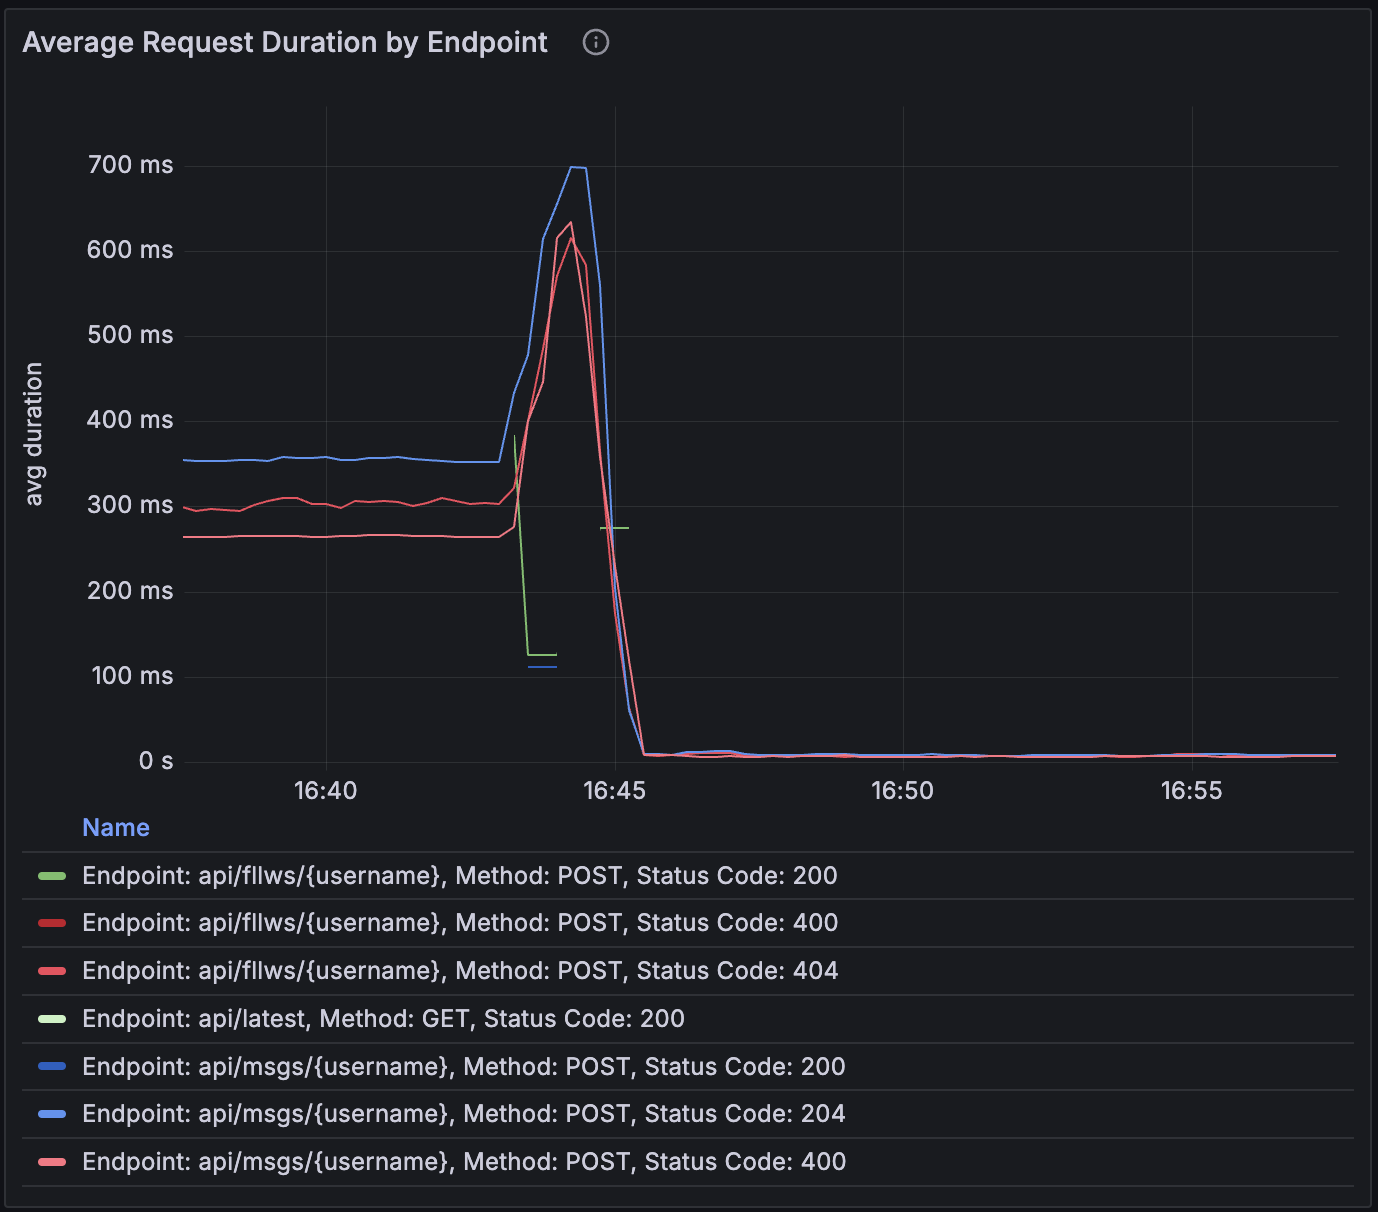
\includegraphics[height=0.9\textwidth]{images/grafana-endpoints-latency.png}
\caption{Significant reduction of latency metrics measured in Grafana}
\label{fig:grafana-endpoints-latency}
\end{figure}

\subsubsection{Grafana and Loki Memory Issues}
We faced disk space overloading on our Grafana server, where Loki was hosted. Using DigitalOcean's recovery console, we identified files deleted but still held open by processes using `sudo lsof +L1`. Terminating these processes with `sudo kill -HUP [PID]` released the disk space (see Figure \ref{fig:grafana-memoryleak}), restored server functionality, and allowed us to regain access to Grafana and SSH, and correctly set up the volume.

Issue Link: \href{https://github.com/DevopsGroupC/Minitwit/wiki/Week-14}{\color{blue}Link for wiki issue week 14}


\begin{figure}[H]
\centering
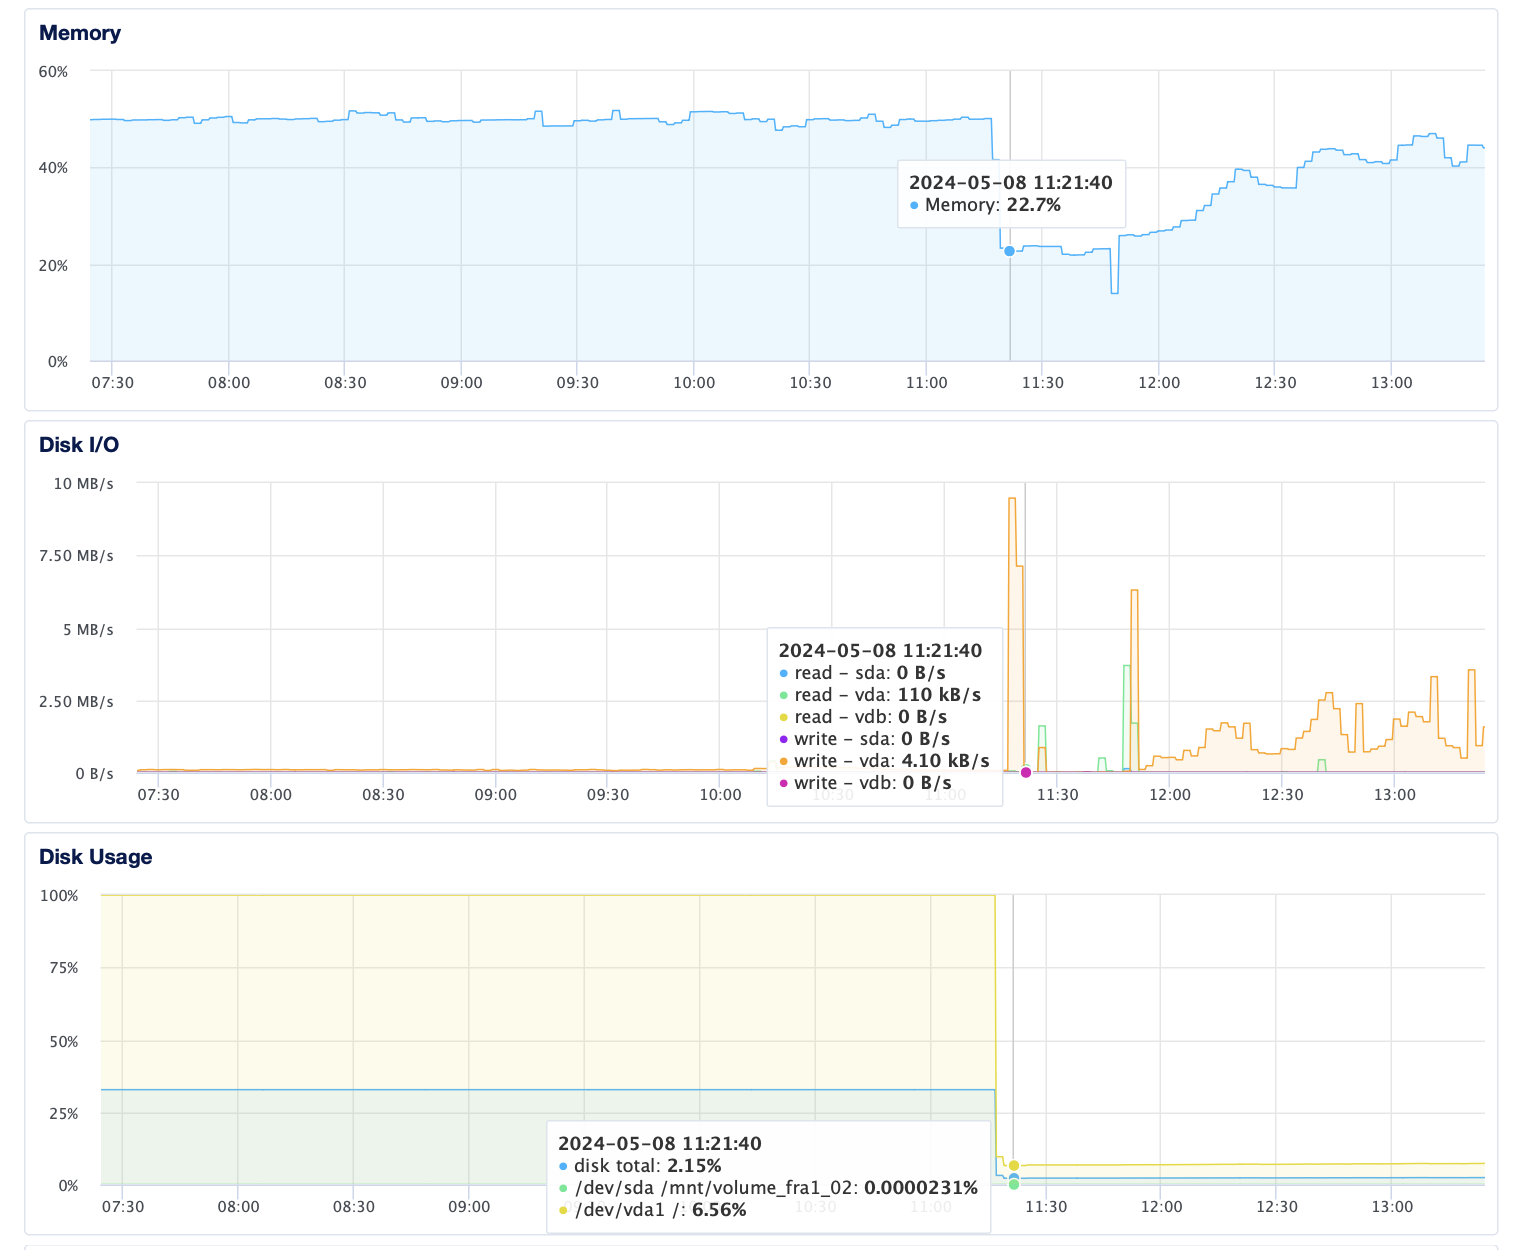
\includegraphics[height=0.9\textwidth]{images/CleanUpMemoryLeakGrafanaServer.png}
\caption{Cleaning up the disk after memory exhaustion}
\label{fig:grafana-memoryleak}
\end{figure}


\subsection{Maintenance}
\subsubsection{Improper Logging Configuration}
Due to the flawed configuration of the volume on the Grafana-server we had a disk overload. At first we tried to resolve this by deleting log files every 12 hours using a cronjob. However, this method was flawed as it deleted files still in use by running processes, resulting in a memory leak. The correct approach was to reconfigure the server to store logs on the attached volume and transfer the existing logs from the disk to this volume.

Issue Link: \href{https://github.com/DevopsGroupC/Minitwit/wiki/Week-14}{\color{blue}Link for wiki issue week 14}

% \subsection{Monitoring - Performance improvements}
% By analyzing metrics, specifically "average request duration by endpoint", and incorporating research conducted by one of the team members, we successfully reduced latency across our endpoints. This improvement is evident in the screenshot below: 
% \begin{figure}[H]
%     \centering
%     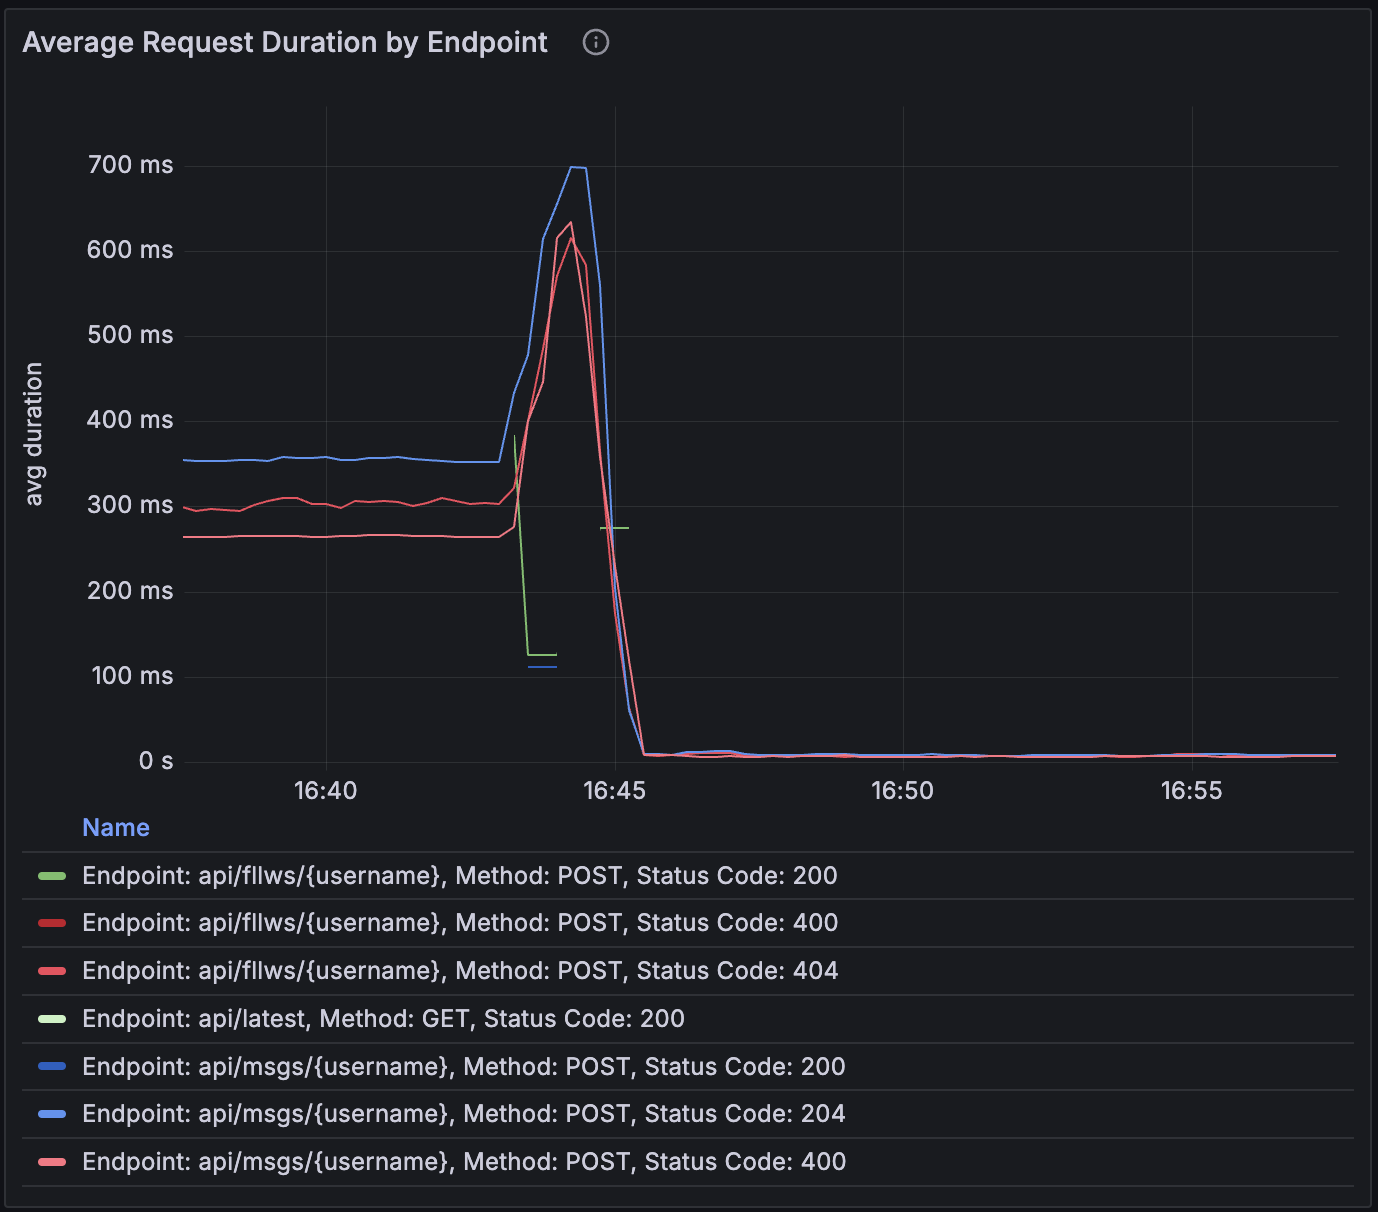
\includegraphics[height=0.9\textwidth]{images/grafana-endpoints-latency.png}
%     \caption{Significant reduction of latency metrics measured in Grafana}
%     \label{fig:grafana-endpoints-latency}
% \end{figure}

% The primary cause of the high latency was the geographical separation between our Database (hosted in the NYC region) and our application server (in the FRA region).

% Issue link: 

% \subsection{Monitoring - Bug fixing}

% The follow/unfollow endpoint was returning a 200(OK) status code, instead of 204(NO CONTENT) as requested by the simulator API, resulting in cumulative errors. It was possible to detect that given the information provided by the \href{http://206.81.24.116/status.html}{\color{blue}http://206.81.24.116/status.html} dashboard. 
% \\
% Issue: Grafana and Loki memory issues
% In addressing the disk space overloading issues on our Grafana server where we hosted Loki as well, we utilized DigitalOcean's recovery console to identify and resolve the root cause. By executing the command $sudo lsof +L1$, we detected files that had been deleted but were still held open by processes, which in turn occupied disk space. We terminated these processes using $sudo kill -HUP [PID]$, which released the disk space and restored server functionality, allowing us to regain access to the Grafana platform and establish SSH connecitons to the server. This intervention resolved the memory issue and retored normal operations.

% Issue link:
% Slow response on the /public endpoint ... ??
% Issue link: \href{https://github.com/DevopsGroupC/Minitwit/issues/141}{\color{blue}Look into adding indices to our database \#141}

\subsection{DevOps Practices Reflection}

Our approach to this project was "DevOps"-oriented compared to previous development projects. Key differences and practices included:
\begin{itemize}
    \item Continuous Monitoring and Feedback: We implemented Grafana and Prometheus, which allowed us to identify and resolve performance issues and bugs.
    \item Infrastructure as Code: We used Terraform for infrastructure management, enabling consistent and repeatable deployments.
    \item Collaboration and Communication: The use of GitHub for issue tracking and commit referencing improved team collaboration.
    \item Automated Testing and Deployment: Our CI/CD pipeline, built using GitHub Actions, reducing the risk of human error and speeding up the release process.
\end{itemize}

\noindent These DevOps practices enhanced our ability to maintain and evolve the CSharp-MiniTwit system efficiently and reliably.
